\documentclass[24pt,pdf,hyperref={unicode},aspectratio=169]{beamer}
\usepackage[utf8]{inputenc}
\usepackage{aiml}

\begin{document}

\section{Генетический алгоритм}

\begin{frame}\frametitle{Генетический алгоритм}
\begin{columns}
\column{0.5\textwidth} 

\begin{itemize}
 \item<2-> Кодирование
 \item<5-> Генерация
 \item<6-> Выбор мутирующих особей
 \item<7-> Мутация
 \item<11-> Выбор скрещивающихся особей
 \item<12-> Скрещивание
 \item<16-> Оценка
 \item<20-> Отбор
\end{itemize}

\column{0.5\textwidth} 

\only<1->{$$
W=\{w_1,\ldots,w_n\}
$$

$$
A\subset W
$$

$$
\sum_{a\in A} a=\sum_{b\in W\setminus A} b
$$}
\only<3-5>{$$
s=\begin{array}{|c|c|c|c|c||c|c|}
\hline
0 & 1 & \alert<8>{1} & 0 & 1 & 1 & 1\\
\hline 
\end{array}
$$}
\only<4>{$$
w_i\in A\Leftrightarrow g[i]=1
$$}
\only<8-10>{$$
\begin{array}{r l}
s= & \begin{array}{|c|c|c|c|c||c|c|}
\hline
0 & 1 & \alert<9>{1} & 0 & 1 & 1 & 1\\
\hline 
\end{array} \\[0.3cm]
\uncover<10>{m(s)=} & \uncover<10>{\begin{array}{|c|c|c|c|c||c|c|}
\hline
0 & 1 & 0 & 0 & 1 & 1 & 1\\
\hline 
\end{array}}
\end{array}
$$}
\only<13-15>{\noindent
$$
\begin{array}{r l}
s_1= & \begin{array}{|c|c|c|c||c|c|}
\hline
 1 & \alert<14-15>{0} & \alert<14-15>{0} & 1 & 1 & \alert<14-15>{1}\\
\hline 
\end{array}\\[0.3cm]

s_2=& \begin{array}{|c|c|c|c||c|c|}
\hline
\alert<14-15>{1} & 0 & 1 & \alert<14-15>{0} & \alert<14-15>{0} & 1\\
\hline 
\end{array}\\[0.3cm]

\uncover<15>{c(s_1,s_2) = }& \uncover<15>{\begin{array}{|c|c|c|c||c|c|}
\hline
 1 & 0 & 0 & 0 & 0 & 1\\
\hline 
\end{array}} \\
\end{array}
$$}
\only<17>{$$
f(A)=\left|\sum_{a\in A} a - \sum_{b\in W\setminus A} b\right|
$$}
\only<18>{$$
f(A)=\left|\sum_{a\in A} a - \sum_{b\in W\setminus A} b\right|^{-1}
$$}
\only<19>{$$
f(A)=\left(1+\left|\sum_{a\in A} a - \sum_{b\in W\setminus A} b\right|\right)^{-1}
$$}
\end{columns}
\end{frame}

\begin{frame}\frametitle{Пропорциональное скрещивание}

\begin{columns}
\column{0.5\textwidth}
$$
\begin{array}{c|c}
$\textnumero$ & Value \\
\hline
1 & 0.5 \\
2 & 0.25 \\
3 & 0.125 \\
4 & 0.125 \\
\end{array}
$$
\column{0.5\textwidth}

\only<2>{
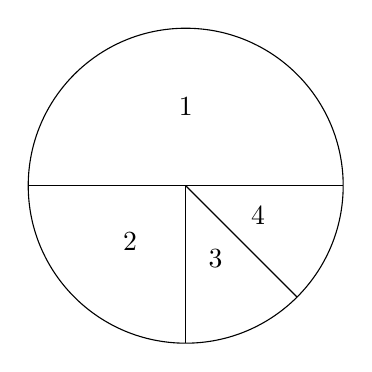
\begin{tikzpicture}
\draw (0,0) circle (2); 
\draw (0,0) -- (2,0);
\draw (0,0) -- (-2,0);
\draw (0,0) -- (0,-2);
\draw (0,0) -- (1.414,-1.414);
\node at (0,1) {1};
\node at (-0.707,-0.707) {2};
\node at (0.92,-0.38) {4};
\node at (0.38,-0.92) {3};

\end{tikzpicture}
}
\end{columns}
\end{frame}

\begin{frame}\frametitle{Элитарное скрещивание}
$$
\begin{array}{l | l l l l l l l l l}
  & 1 & 2 & 3 & 4 & 5 & 6 & 7 & 8 & 9 \\
\hline
1 &   & X & X & X & X & X & X & X & X \\
2 &   &   & X & X & X & X & X &   &   \\
3 &   &   &   & X & X &   &   &   &   \\
4 &   &   &   &   & X &   &   &   &   \\
\end{array}
$$
\end{frame}


\section{Примеры задач}

\begin{frame}\frametitle{Задача коммивояжера}

\uncover<+->{
Дано: граф $G=(V,E)$ и функция $W:E\rightarrow\mathbb{R}$.\\[0.3cm]

Найти: проходящий единожды по всем вершинам цикл $C=(e_1,\ldots,e_n)$ такой, что $\sum_{e\in C} W(e)\rightarrow \min$\\[0.3cm]
}

\uncover<+->{Кодирование: }\uncover<+->{$S: V\rightarrow V$, биекция (перестановка)}\\[0.3cm]

\uncover<+->{Мутация:}\uncover<+->{перестановка соседних элементов}\\[0.3cm]

\uncover<+->{Скрещивание:}

\uncover<+->{$$
c(S_1,S_2)=S_1\circ S_2
$$}

\uncover<+->{Оценка: }\uncover<+->{$$
f(C)=\left(\sum_{e\in C} W(e)\right)^{-1}
$$}

\end{frame}

\begin{frame}\frametitle{Система уравнений}

\uncover<+->{
Дано: система уравнений вида $\left\{ f_i(x_1,\ldots,x_n)=0\right.$, например:

$$
\left\{\begin{array}{c c c}
        x_1^2 + \sin x_2 & = &0 \\
        e^{x_1+x_2}-x_1x_2 & = & 0 \\
       \end{array}\right.
$$

Найти: решение системы уравнений\\[0.3cm]
}

\uncover<+->{Кодирование: }\uncover<+->{$(x_1,\ldots,x_n)$}\\[0.3cm]

\uncover<+->{Мутация: }\uncover<+->{$(c_1x_1,\ldots,c_nx_n)$, $c_i\in[1-\varepsilon,1+\varepsilon]$}\\[0.3cm]

\uncover<+->{Скрещивание: }\uncover<+->{обычное}\uncover<+->{, или $\frac{(x_1,\ldots,x_n)+(y_1,\ldots,y_n)}{2}$}

\uncover<+->{Оценка: }\uncover<+->{$$
\left(1+\sum_{i=0}^{n}\left|f_i(x_1,\ldots,x_n)\right|\right)^{-1}
$$}



\end{frame}




\end{document}